\section{Integrated Development Environment}
The application is written using Android Studio. Android Studio is an \acrshort{ide} supported by Google and based on the IntelliJ \acrshort{ide} of JetBrains, a company that develops an \acrshort{ide} for the most popular general purpose programming languages \cite{AndroidDevelopers2019c}.
\section{General Data Protection Regulation}
The General Data Protection Regulation of the \acrfull{eu} is a measure against possible theft of personal data and the protection of privacy, incorporated by the \acrshort{eu} and its member states in 2016. The general changes regarding the privacy directive of the \acrshort{eu} - firstly declared in 1995 - are as follows \cite{THEEUROPEANPARLIAMENTANDTHECOUNCILOF1995} \cite{EUGDPRPortal:byTrunomi2019}:
\begin{itemize}
\item Test
\end{itemize}

The application that is developed needs to take this specific regulation into account when it handles the personal data of a patient and the employees of the hospital. 
\section{Android Architecture}
\subsection{Testing}
\subsubsection{Testing Workflow}
70-20-10 rule
Red-green bar mantra is used by Google as the main testing workflow. First a failing test is written, then the code to pass the test is developed. After this process needed refactors are applied to the codebase.
\begin{figure}
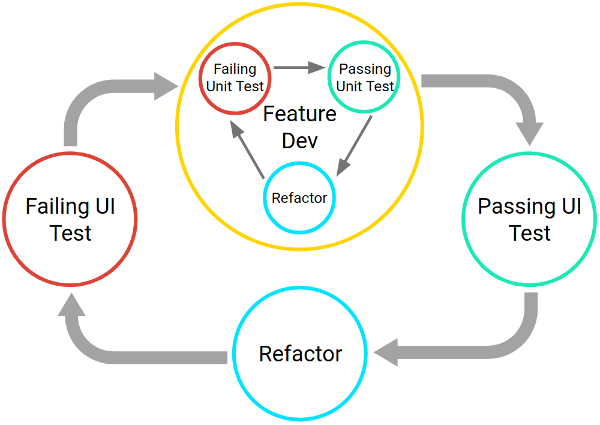
\includegraphics[scale=0.5]{testing-workflow}
\centering
\caption{Testing workflow~\cite{Google_testing2017}}
\end{figure}
\begin{figure}[h!]
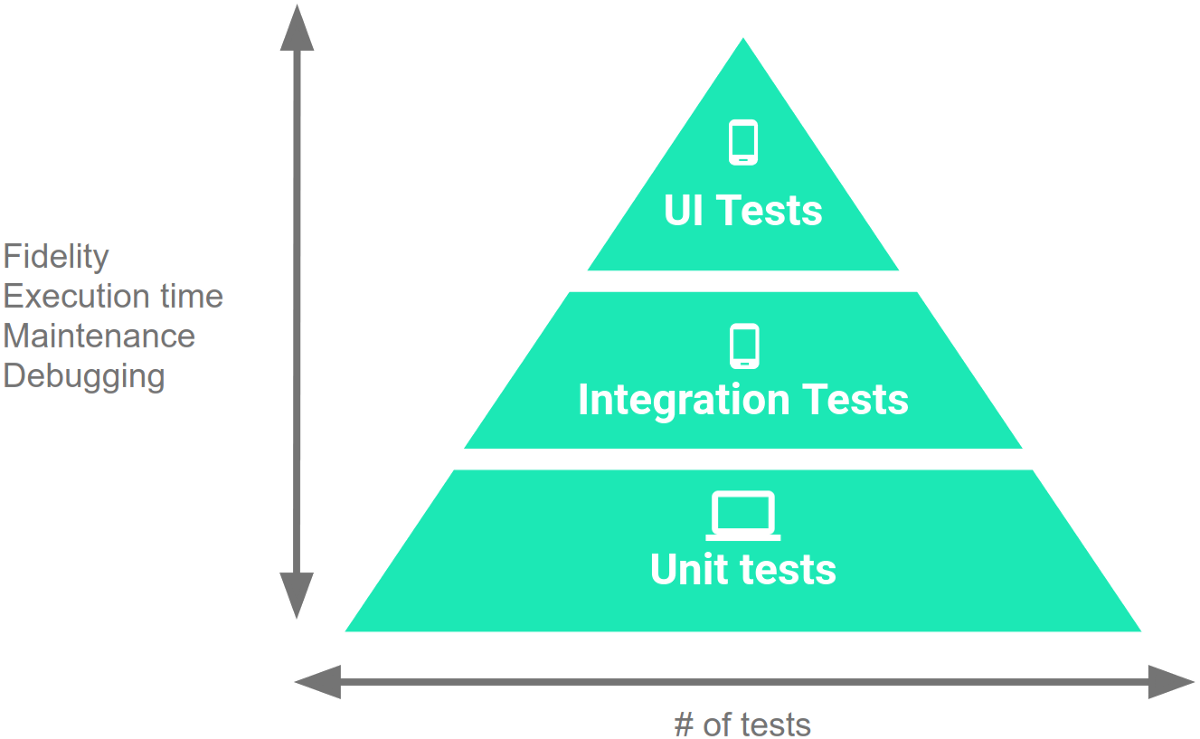
\includegraphics[scale=0.25]{testing_android}
\centering
\caption{Testing pyramid~\cite{FernandoSproviero2018}}
\end{figure}
\subsubsection{Unit Testing}
These tests are responsible for the smaller parts of the application (units) and use mocked or stubbed properties. This means that the properties and methods do not interfere with code written inside the main application. These tests are the fastest in runtime (compared to the integration and UI testing) because they do not need a running device or emulator, which means they are the least expensive to execute. Some testing frameworks from Android are: JUnit4 and Mockito (Mockito is used to create mock instances of dependencies, classes, properties and methods) \cite{FernandoSproviero2018}. The characteristics of a good unit test are \cite{Google_testing2017}:
\begin{enumerate}
\item Thorough;
\item Focused;
\item Repeatable;
\item Fast;
\item Verifies behaviour;
\item Concise;
\end{enumerate}
\subsubsection{Integration Testing}
These tests test the interaction between different units of the application. The tests do not cover any updates on the UI thread and test the units independently from the UI. A common framework used to write integration tests is Roboelectric \cite{Roboelec2019}. When an application is in development the integration tests will check the behaviour of the different interacting units when the new feature is implemented. This way, the development team can roll-out features without breaking the current application.
\subsubsection{User Interface Testing}
\subsection{Separation of concern: Dependency Injection}
Separation of concern is a general convention amongst software developers. In practice it is harder to implement than it first seems. One of the core components of this pattern are dependencies: one class depends on the structure of another class. The dependency pattern enables developers to focus on their code without having to worry about the dependency. For a class it is enough to know how a dependency is structure, there is no need for the class to know how it is implemented. This is also the last of the SOLID principles, the principle of dependency on abstraction instead of concrete implementation \cite{BhavyaKaria2018}.
\subsubsection{Dependency Injection: Restaurant Analogy}
To comprehend the concept of dependency injection let's have a look at a fairly common analogy". A man comes into a restaurant and takes a look at the menu. After having taken a close look, the man decides to order fish and chips. The waiter notifies the kitchen and tells the head chef that a customer ordered the fish and chips. Upon finishing the plating, the waiter brings the wonderful plate of fish and chips to the customer (the man). The man obtained what he wanted without knowing how his dish was prepared, the head chef knew what the customer needed and provided the meal.
\subsubsection{Benefits of using Dependency Injection}
Using dependency injection might seem somewhat bloated in practice, but there are some enormous benefits upon applying this pattern on an application. Some of these benefits are listed below \cite{Seemann2011}:
\begin{itemize}
\item Late binding: interchangeable services;
\item Extensibility: reusable code;
\item Maintainability: classes with a well-defined responsibility become easier to maintain;
\item Testability: classes having a dependency can be tested separately - as a single unit; 
\item Enforces usage of loose coupling;
\end{itemize}
\subsubsection{Types of Dependency Injection}
Constructor injection is the type of DI (dependency injection) that uses a private field for the dependency and sets this field using a parameter inside of the constructor. Setter (property) injection uses a property of the class that requires the dependency and works via getter and setter methods. The dependency is individually set instead of passed as a parameter in the constructor. This is quite easy to understand but hard to implement in a robust way, this only works if the value passed in the setter is a good value. When dependencies are only used in specific methods, it might be easier to just pass them as parameters to that method, this is called method injection. This way of implementing DI is also simple and straightforward \cite{TheoJungeblut2015}.
\subsection{Lifecycle Events}
For the duration of the runtime of the mobile application (from the moment the app is opened until it is closed) some events occur that are typical for an Android mobile application. A brief summary of these events is listed below (in chronological order) \cite{AndroidDeveloper2019}:
\begin{itemize}
\item onCreate() - When the activity is launched (This can happen after the onDestroy() event);
\item onStart() - When the activity is visible to the user;
\item onResume() - When the user returns to the activity after an onPause() event occurs;
\item onPause() - When activity is no longer visible;
\item onStop() - When the activity is finished or destroyed;
\item onRestart() - When the activity is restarted after a stoppage;
\item onDestroy() - When the activity is shut down;
\end{itemize}
\begin{figure}[H]
\centering
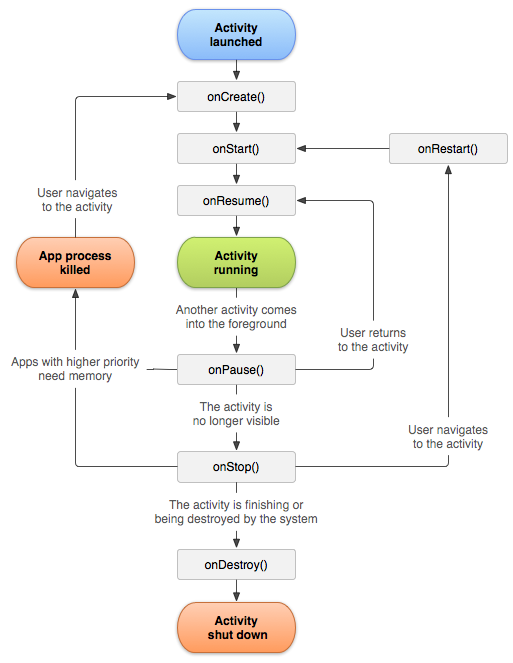
\includegraphics[scale=0.5]{activity_lifecycle}
\caption{Android Activity Lifecycle Schematic~\cite{AndroidDeveloper2019}}
\end{figure}
The lifecycle of an activity is an important factor to take into account whilst the application is being developed. This means a certain level of persistency is required for an optimal user experience.
\subsubsection{Bundles \& Saved State}
The way in which the onCreate() method is implemented allows a developer to declare a Bundle, which is an object that contains key-value pairs, that is used to restore an activity's previous state. If no such state exists then the Bundle will be equal to null. The Bundle object that is passed to an activity in the onCreate() method should only contain specific information such as user interactions: form fields, position on the screen and sometimes navigational properties. The main usage for this technology is when an activity gets paused or stopped, this means the OS (operating system) can freely destroy any activities \cite{JamesHalpern2012}.
\subsection{Offline storage and persisting data}
Another way to persist data throughout the lifecycle of an application is to use the (smart)phone's local storage. Each application can create a new local database using SQLite. SQLite is a transactional and file-based database (db), which means it is optimal for storing user-specific data. The fact that it is indeed a transactional db means that upon failure of an operation it will roll-back to the previous state and revert all existing, pending changes \cite{TutorialsPoint2019}.
\subsection{Repository Design Pattern}
A common pattern to use for handling database communication the repository pattern. This pattern acts as an abstraction layer on top of the data layer and the business layer and centralises the domain models. One of the common ways of integrating the pattern is creating a \acrfull{dao} that interacts with the database of the application and a repository that can pass data from and to the \acrshort{dao}. Using the pattern as an additional abstraction layer enables easier testing and enforces the single responsibility principle \cite{Per-ErikBergman2017} \cite{NahidulHasan2018}.
\subsubsection{RoomDB}
A nice feature from the Android SDK is a wrapper for SQLite inside the app: RoomDB. RoomDB is a feature set for SQLite statement and works using the repository pattern. The interaction between the application (view layer) and data layer happens using a repository which can be implemented locally (offline storage using the RoomDB wrapper) as well as remotely (remote API calls). The structure of the application is as follows:
\begin{figure}[h!]
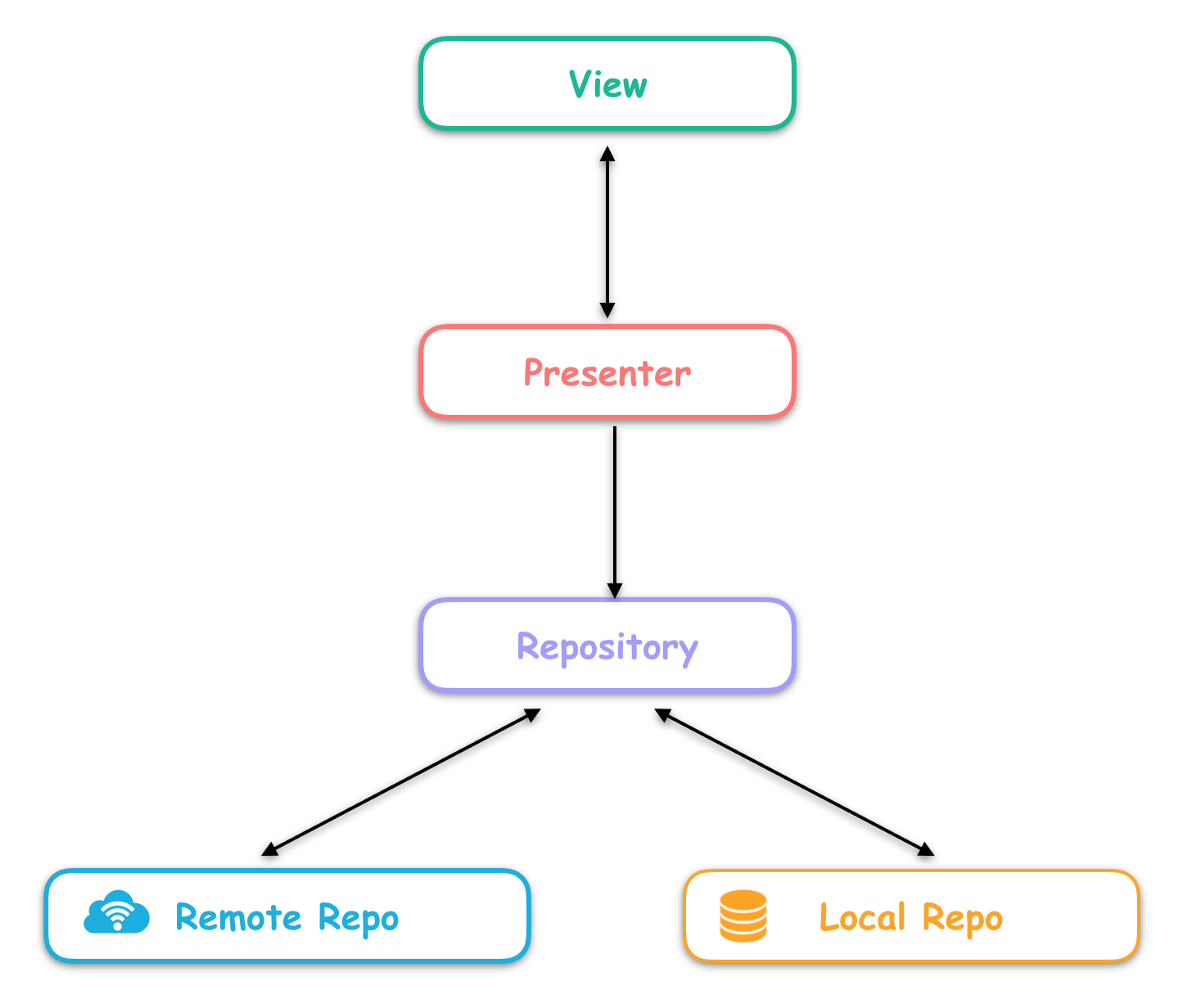
\includegraphics[scale=0.25]{repository_pattern_android}
\centering
\caption{Repository Pattern inside an android application~\cite{EslamHussein2018}}
\end{figure}
\begin{figure}[h!]
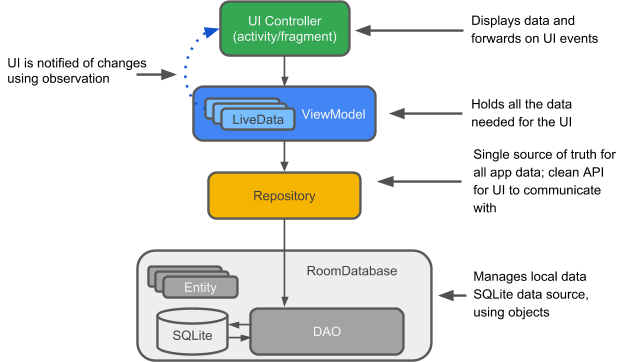
\includegraphics[scale=0.5]{local_repo_android}
\centering
\caption{Local repository usage inside the app~\cite{Unknown2018}}
\end{figure}
\subsection{Model - View - ViewModel Architecture}
One of the downsides of the default architecture of an Android application is the interaction between a view, model and layout files. Normally an activity is created with corresponding models which data needs to be presented in the view. This results in , possibly, a very large activity or fragment class. A good practice is to implement a Model-View-ViewModel architecture, which focuses on separating the different components required to generate a view, thus following the separation of concern principle. This principle is one that every developer should take into account, because it is the most important one. The prime advantage of using this principle is that is easier to maintain and opts for more testable components of your application \cite{AndroidDevelopers2019b}.
\subsubsection{UI Driven}
The optimal way of building an application is making the \acrshort{ui} dependent of a model, a class holding the data for a corresponding entity, preferably persistent. A model acts independently of an activity's or fragment's lifecycle and consequently independently of the concerns regarding handling lifecycles.
\subsubsection{Interaction between ViewModel - View}
An easy way of incorporating the viewmodel is via the ViewModelProvider class, which returns a reference to the ViewModel class specified. This viewmodel contains data that will drive the \acrshort{ui} and methods that will handle business logic. Typically the ViewModel has a LiveData list of the type of model that needs to be used and some references to a local and remote repository to fetch the data in an asynchronous fashion. The difficulty is to create a reactive \acrshort{ui}, that handles any changes to the data in the ViewModel object \cite{JaewoongEum2018}.
\subsubsection{LiveData and observables}
LiveData is a datatype that is lifecycle aware, meaning it will can monitor changes and notifies the \acrshort{ui} when that happens. The benefit of this datatype is the absence of any additional and rigid logic to handle the data binding. Methods returning LiveData can be observed using the observable pattern, the method is called from the ViewModel object and observed for changes in the LiveData that is returned by the method. This enables data-binding by only applying minor changes to the code inside the ViewModel and View \cite{AndroidDevelopers2019b}.
\begin{figure}[h!]
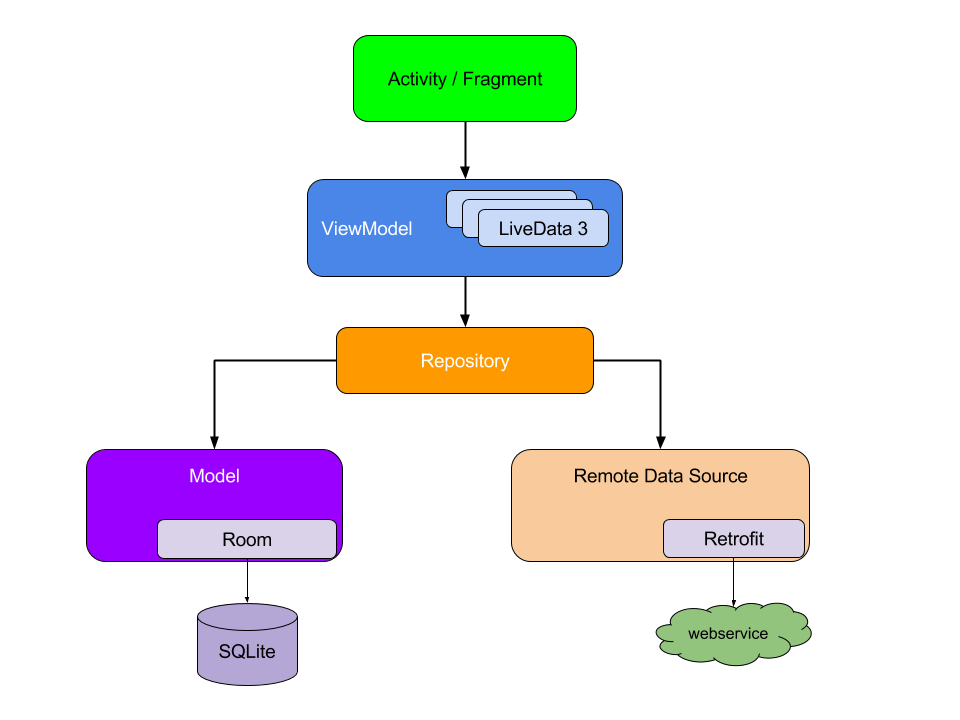
\includegraphics[scale=0.4]{app_architecture}
\centering
\caption{Complete architecture of application using ~\acrshort{mvvm}~\cite{AndroidDevelopers2019b}}
\end{figure}